\documentclass{article}
\usepackage[margin=1in]{geometry}
\usepackage{graphicx}
\usepackage{hyperref}
\title{\vspace{-2.0cm}ViReport v0.0.1}
\author{Niema Moshiri}
\date{2020-03-02}
\begin{document}
\maketitle

\section{Input Dataset}
The analysis was conducted on a dataset containing 179 sequences.
The average sequence length was 29800.234636871508,
with a standard deviation of 407.74200508520295.
The earliest sample date was 2013-07-24,
the median sample date was 2020-01-23,
and the most recent sample date was 2020-02-28.


\begin{figure}[h]
\centering
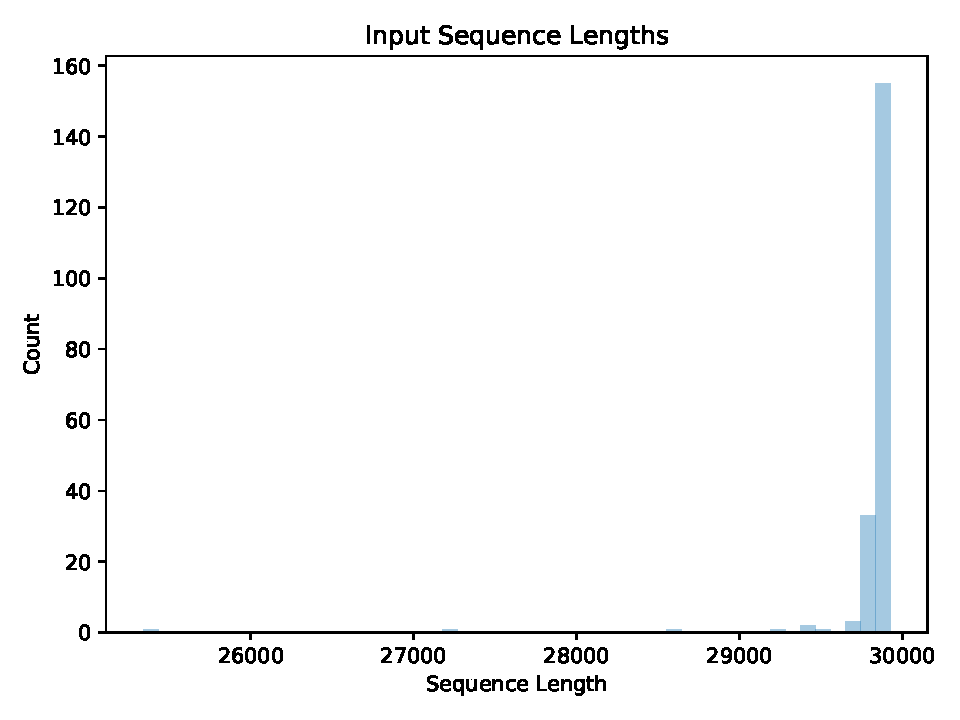
\includegraphics[width=0.75\textwidth]{./figs/input_sequence_lengths.pdf}
\caption{Distribution of input sequence lengths}
\end{figure}



\begin{figure}[h]
\centering
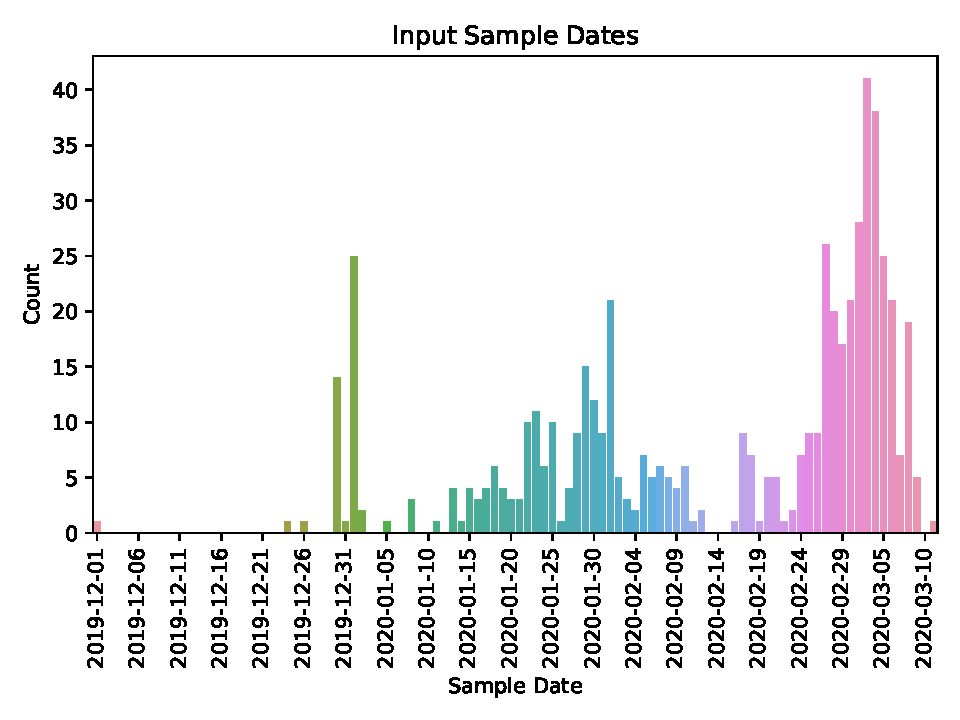
\includegraphics[width=0.75\textwidth]{./figs/input_sample_dates.pdf}
\caption{Distribution of input sample dates}
\end{figure}

\section{Preprocessed Dataset}
The input dataset was preprocessed such that sequences were given safe names: non-letters/digits in sequence IDs were converted to underscores.
After preprocessing, the dataset contained 179 sequences.
The average sequence length was 29800.234636871508,
with a standard deviation of 407.74200508520295.
The earliest sample date was 2013-07-24,
the median sample date was 2020-01-23,
and the most recent sample date was 2020-02-28.


\begin{figure}[h]
\centering
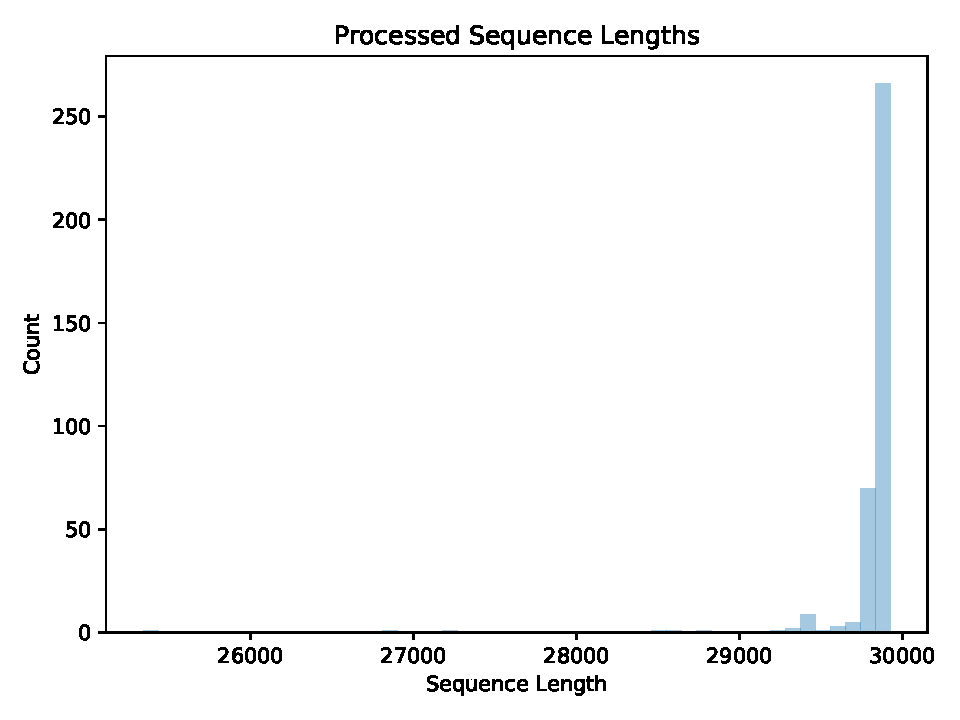
\includegraphics[width=0.75\textwidth]{./figs/processed_sequence_lengths.pdf}
\caption{Distribution of preprocessed sequence lengths}
\end{figure}



\begin{figure}[h]
\centering
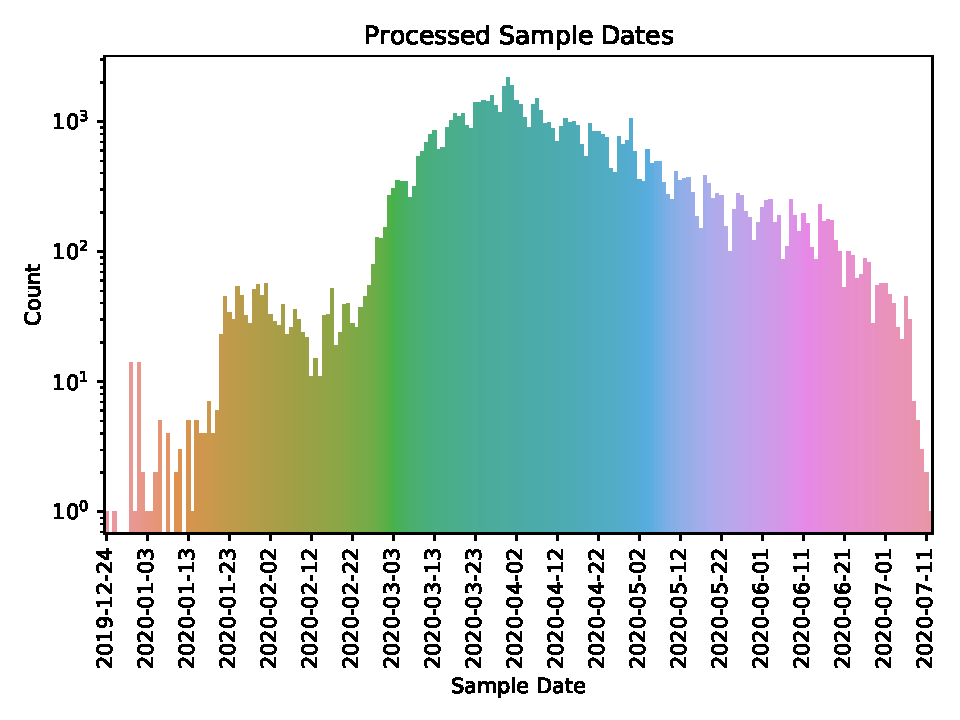
\includegraphics[width=0.75\textwidth]{./figs/processed_sample_dates.pdf}
\caption{Distribution of preprocessed sample dates}
\end{figure}

\section{Multiple Sequence Alignment}
Multiple sequence alignment was performed using MAFFT (Katoh \& Standley, 2013) in automatic mode.
There were 30379 positions (16956 invariant) and 157 unique sequences in the multiple sequence alignment.
Pairwise distances were computed from the multiple sequence alignment using the tn93 tool of HIV-TRACE (Pond et al., 2018).
The average pairwise sequence distance was 0.0002367379605663574,
with a standard deviation of 0.0002469060445309071.


\begin{figure}[h]
\centering
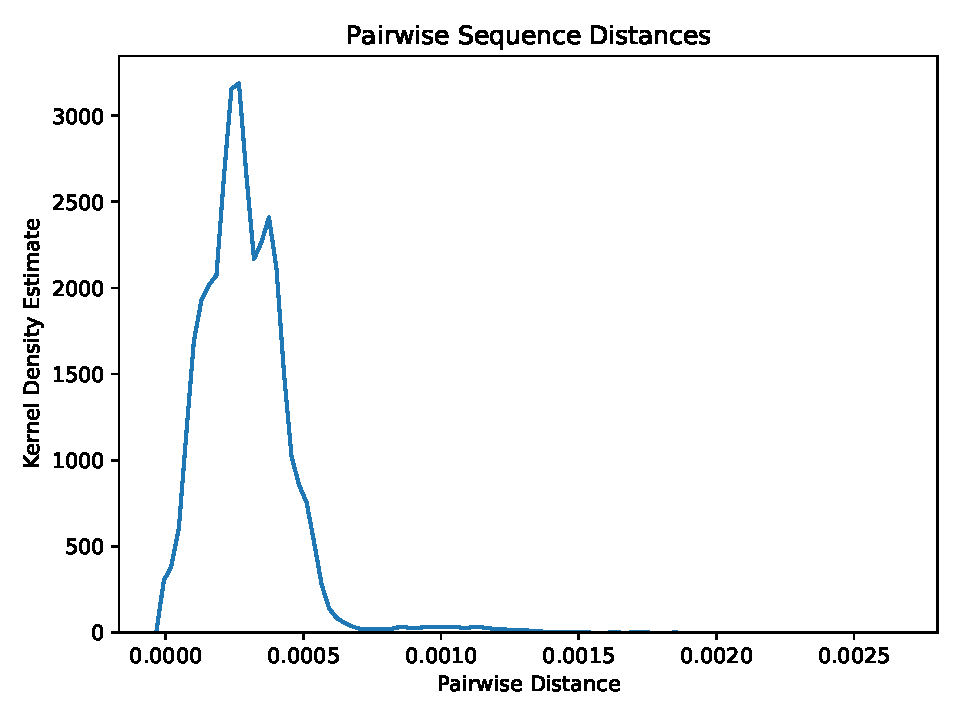
\includegraphics[width=0.75\textwidth]{./figs/pairwise_distances_sequences.pdf}
\caption{Distribution of pairwise sequence distances}
\end{figure}

\section{Phylogenetic Inference}
A maximum-likelihood phylogeny was inferred under the General Time-Reversible (GTR) model (Tavare, 1986) using FastTree 2 (Price et al., 2010) using a Gamma20-based likelihood.
The inferred phylogeny was MinVar-rooted using FastRoot (Mai et al., 2017).
Pairwise distances were computed from the phylogeny using TreeSwift (Moshiri, 2020).
The maximum pairwise phylogenetic distance (i.e., tree diameter) was 0.0035765329999999976,
and the average pairwise phylogenetic distance was 0.00040441892561284877,
with a standard deviation of 0.0004151634456449567.


TODO INSERT ROOTED TREE VISUALIZATION HERE




\begin{figure}[h]
\centering
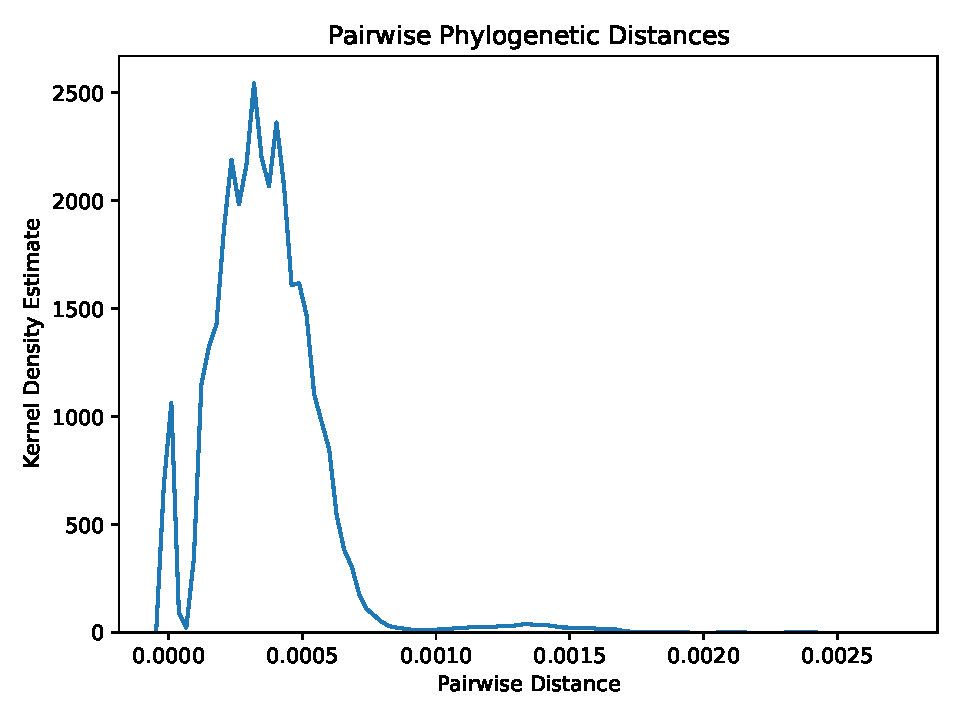
\includegraphics[width=0.75\textwidth]{./figs/pairwise_distances_tree.pdf}
\caption{Distribution of pairwise phylogenetic distances}
\end{figure}

\section{Phylogenetic Dating}
The rooted phylogeny was dated using treedater (Volz \& Frost, 2017).
The height of the dated tree was 255.11532509799997 days,
so given that the most recent sample was collected on 2020-02-28,
the estimated time of the most recent common ancestor (tMRCA) was 2019-06-17.


TODO INSERT DATED TREE VISUALIZATION HERE


\section{Transmission Clustering}
Transmission clustering was performed using TreeN93 (Moshiri, 2018) using pairwise phylogenetic distances.
The total number of singletons (i.e., non-clustered individuals) was 111,
and the total number of clusters (excluding singletons) was 19.
The average cluster size (excluding singletons) was 3.0526315789473686,
with a standard deviation of 1.0989796325169001,
and the maximum and minimum cluster sizes were 5 and 2, respectively.


\begin{figure}[h]
\centering
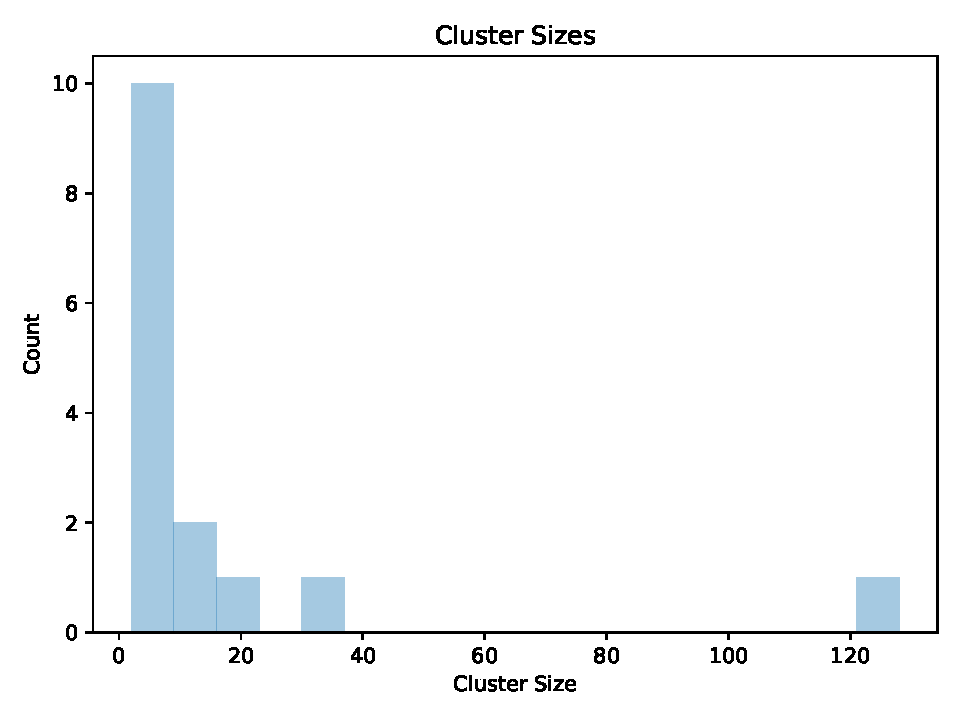
\includegraphics[width=0.75\textwidth]{./figs/cluster_sizes.pdf}
\caption{Distribution of cluster sizes (excluding singletons)}
\end{figure}


\end{document}
